%% chapters/chapter_1.tex
%%
%% Copyright 2017 Evandro Coan
%% Copyright 2012-2014 by abnTeX2 group at http://abntex2.googlecode.com/
%%
%% This work may be distributed and/or modified under the
%% conditions of the LaTeX Project Public License, either version 1.3
%% of this license or (at your option) any later version.
%% The latest version of this license is in
%%   http://www.latex-project.org/lppl.txt
%% and version 1.3 or later is part of all distributions of LaTeX
%% version 2005/12/01 or later.
%%
%% This work has the LPPL maintenance status `maintained'.
%%
%% The Current Maintainer of this work is the Evandro Coan.
%%
%% The last Maintainer of this work was the abnTeX2 team, led
%% by Lauro César Araujo. Further information are available on
%% https://www.abntex.net.br/
%%
%% This work consists of a bunch of files. But originally there were 2 files
%% which are renamed as follows:
%% Deleted the `abntex2-modelo-img-marca.pdf`
%% Renamed the `abntex2-modelo-include-comandos.tex, v-1.9.2 laurocesar` to `chapters/chapter_1.tex`
%%
% ---
% Este capítulo, utilizado por diferentes exemplos do abnTeX2, ilustra o uso de
% comandos do abnTeX2 e de LaTeX.
% ---

% The \phantomsection command is needed to create a link to a place in the document that is not a
% figure, equation, table, section, subsection, chapter, etc.
% https://tex.stackexchange.com/questions/44088/when-do-i-need-to-invoke-phantomsection
\phantomsection

% https://tex.stackexchange.com/questions/5076/is-it-possible-to-keep-my-translation-together-with-original-text
\chapter[\lang{Algorithms Presentation}{Algoritmos de calibração utilizados}]
{
    \lang
    {Calibration Algorithms used}
    {Algoritmos de calibração utilizados}
}

\label{cap_algoritmos}


%\begin{flushright}
%    \englishword{\showfont}
%\end{flushright}

% Why latex is letting my text goes out of the screen?
% https://tex.stackexchange.com/questions/386762/why-latex-is-letting-my-text-goes-out-of-the-screen
%\sloppy
%\textbf{textbf: \englishword{\showfont}}
%\fussy


\section{Linearização por mínimos quadrados ordinários - \textit{Ordinary Least Squares}}

Este primeiro método baseia-se no princípio dos mínimos quadrados para obtenção dos parâmetros desconhecidos (ou coeficientes) de um modelo de regressão linear: minimizar a soma dos quadrados das diferenças entre os valores observados em determinado conjunto de dados e os valores preditos pela função linear da variável independente.

De forma geométrica, este método pode ser visto como a soma das distâncias ao quadrado entre cada ponto no grupo de dados adquiridos e o seu ponto correspondente na função de regressão. Quanto menor essa distância, melhor o modelo se ajusta aos dados.

Para compreender o método matematicamente, partimos da definição de regressão linear, pois este conceito é importante não apenas para o método de Mínimos quadrados ordinários, mas para a compreensão de todos os outros métodos citados neste trabalho: regressão linear é um modelo estatístico utilizado para estimar o valor esperado de uma variável \textit{y}, dados os valores de outras variáveis \textit{x}, através da seguinte fórmula \cite{ols_intro_econometrics}:

\begin{equation}\label{eq:1}
y_i = \alpha + \beta x_i + \epsilon_i
\end{equation}

Onde \textit{y} é a variável a ser estimada, \textit{x} é a variável que deverá ser capaz de estimar \textit{y}, $\alpha$ é o parâmetro independente de \textit{x} e  $\beta$ é o coeficiente da variável \textit{x}. No caso em estudo, onde existem \textit{n} amostras a serem utilizadas nessa linearização, \textit{x} e \textit{y} serão vetores de tamanho \textit{n}.

Graficamente, essa linearização pode ser exemplificada pela figura \ref{fig:ols_1}, que ilustra cada um dos termos da equação, bem como a própria linha regressora:

\begin{figure}[htp]
    \centering
    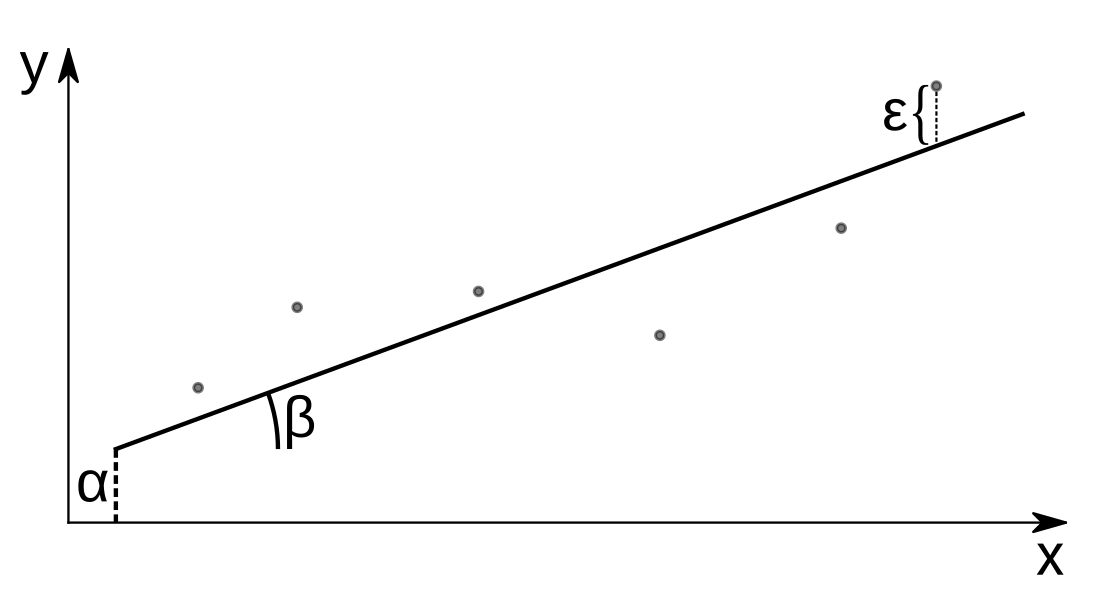
\includegraphics[width=12cm]{lsq.png}
    \caption{Representação gráfica da linearização por mínimos quadrados ordinários}
    \label{fig:ols_1}
\end{figure}

Matricialmente, a equação \ref{eq:1} pode ser exposta da forma:

\begin{equation*} \textbf{Y}= \alpha + \textbf{X}\beta+\epsilon, \end{equation*}

Onde \textbf{Y} representa o vetor de valores a serem estimados, \textbf{X} representa o vetor de dados observados, $\beta$ e $\alpha$ os coeficientes dependentes e independentes respectivamente, e $\epsilon$ um vetor ou matriz de erros com variâncias constantes, da forma:

\begin{equation*} \left(\begin{array}{cccc} \sigma^{2} & 0 & \ldots & 0 \\ 0 & \sigma^{2} & \ldots & 0 \\ \vdots & \vdots & \ddots & \vdots \\ 0 & 0 & \ldots & \sigma^{2} \\ \end{array} \right) \end{equation*}

O objetivo do método de mínimos quadrados ordinários é encontrar as estimativas de $\beta$ e $\alpha$ e isto é feito à partir da minimização da soma dos quadrados dos erros $e_i$, ou seja:

\begin{equation}\label{eq:2}
S(\alpha, \beta) =\arg\min_{\beta}\sum_{i=1}^{n}\epsilon_{i}^{2}\\ 
\end{equation}

A ideia por trás dessa técnica é que, minimizando a soma do quadrado dos erros, sejam obtidos $\beta$ e $\alpha$ que trarão a menor diferença entre a estimativa de \textit{y}  e o valor de \textit{y} realmente observado. 

Para prosseguir no desenvolvimento do método, é substituído $e_i$ por $y_i - \alpha - \beta x_i$, da forma:

\begin{equation}\label{eq:3}
S(\alpha, \beta) = \sum_{i=1}^{n} (y_i - \alpha - \beta x_i)^2
\end{equation}

A minimização ocorre com a derivação via regra da cadeia de $S(\alpha, \beta)$ em relação à $\alpha$ e $\beta$ e igualando esse resultado a zero, como é mostrado abaixo:

\begin{equation*} 
\frac{\delta S}{\delta \alpha} = \frac{\delta S}{\delta x_i} \ast \frac{\delta x_i}{\delta \alpha}
\end{equation*}

\begin{equation*}
\frac{\delta S}{\delta x} = 2 \sum_{i=1}^{n} (y_i - \alpha - \beta x_i)
\end{equation*}

\begin{equation*}
\frac{\delta x_i}{\delta \alpha} = -1
\end{equation*}

\begin{equation}\label{eq:4}
\frac{\delta S}{\delta \alpha} = -2 \sum_{i=1}^{n} (y_i - \alpha - \beta x_i) = 0
\end{equation}

\begin{equation}\label{eq:5}
\frac{\delta S}{\delta \beta} = -2 \sum_{i=1}^{n} x_i (y_i - \alpha - \beta x_i) = 0
\end{equation}

Dividindo a equação \ref{eq:4} por 2n, é obtido:

\begin{equation*}
 \frac {-\sum_{i=1}^{n}y_i}{n} + \frac{\sum_{i=1}^{n}\alpha}{n} + \frac{\sum_{i=1}^{n}\beta x_i}{n} = 0
\end{equation*}

Que pode ser reescrito da forma:

\begin{equation*}
 - \overline{y} + \alpha + \beta \overline{x} = 0 
\end{equation*}

\begin{equation}\label{eq:6}
\overline{y}  = \alpha + \beta \overline{x} 
\end{equation}

Onde $\overline{x}$ e $\overline{y}$ representam as médias amostrais de \textit{x} e \textit{y}, respectivamente.

Substituindo esse resultado na equação \ref{eq:5}:

\begin{equation*}
-2 \sum_{i=1}^{n} x_i (y_i - \overline{y} + \beta \overline{x} - \beta x_i) = 0
\end{equation*}

\begin{equation*}
\sum_{i=1}^{n}[x_i (y_i - \overline{y}) + x_i \beta (\overline{x} - x_i)] = 0
\end{equation*}

\begin{equation*}
\sum_{i=1}^{n} x_i (y_i - \overline{y}) + \beta \sum_{i=1}^{n} x_i  (\overline{x} - x_i) = 0
\end{equation*}

Isolando $\beta$:

\begin{equation}\label{eq:7}
\beta = \frac{\sum_{i=1}^{n} x_i (y_i - \overline{y})}{\sum_{i=1}^{n} x_i(\overline{x} - x_i)}
\end{equation}

Após o cálculo de $\beta$, basta reorganizar a equação \ref{eq:6} para obter $\alpha$:

\begin{equation}\label{eq:8}
  \alpha = \overline{y} - \beta \overline{x} 
\end{equation}

Para a obtenção resultados ótimos utilizando este método, algumas premissas devem ser consideradas:

\begin{itemize}
  \item Os regressores \textit{x} devem ser fixos, isto é, o vetor \textit{X} não deve ser estocástico;
  \item O erro deve ser aleatório e com média igual à zero, ou seja: $E(\epsilon) = 0$;
  \item O erro deve ser distribuído conforme a curva normal;
  \item Não deve haver correlação entre os erros das amostras;
  \item A variância do erro deverá ser constante, isto é, as variáveis deverão ser homoscedásticas;
  \item Os parâmetros desconhecidos $\alpha$ e $\beta$ deverão ser constantes;
  \item Os dados da variável dependente $y$ deverão ser gerados pela função linear $y = X\beta + \alpha + \epsilon$;
\end{itemize}

Uma das principais medidas de qualidade deste método em relação à sua capacidade de estimar corretamente os valores de \textit{y} é o coeficiente de determinação $R^2$ \cite{ols_intro_econometrics} \cite{conciseenclyclopediaofstatistics}. A equação para obtenção deste coeficiente é vista abaixo:

\begin{equation}\label{eq:9}
R^2 = 1 - \frac{\sum_{i=1}^{n} y_i(\beta x_i + \alpha)^2}{\sum_{i=1}^{n} (y_i - \overline{y})^2}
\end{equation}

$R^2$ varia de 0 a 1 e quanto mais próximo de 1, melhor o método estima os valores de \textit{y}.

\section{Linearização por mínimos quadrados ponderados - \textit{Weighted Least Squares}}

Uma das pressuposições do modelo de linearização por mínimos quadrados ordinários é que a variância do erro entre as amostras deve ser constante, isto é, que as variáveis em análise devem ser homoscedásticas. Entretanto, nem sempre essa suposição é atendida. Na figura \ref{fig:outlier}, é possível observar um conjunto de amostras com variância constante e outro com variância não constante.

\begin{figure}[htp]
    \centering
    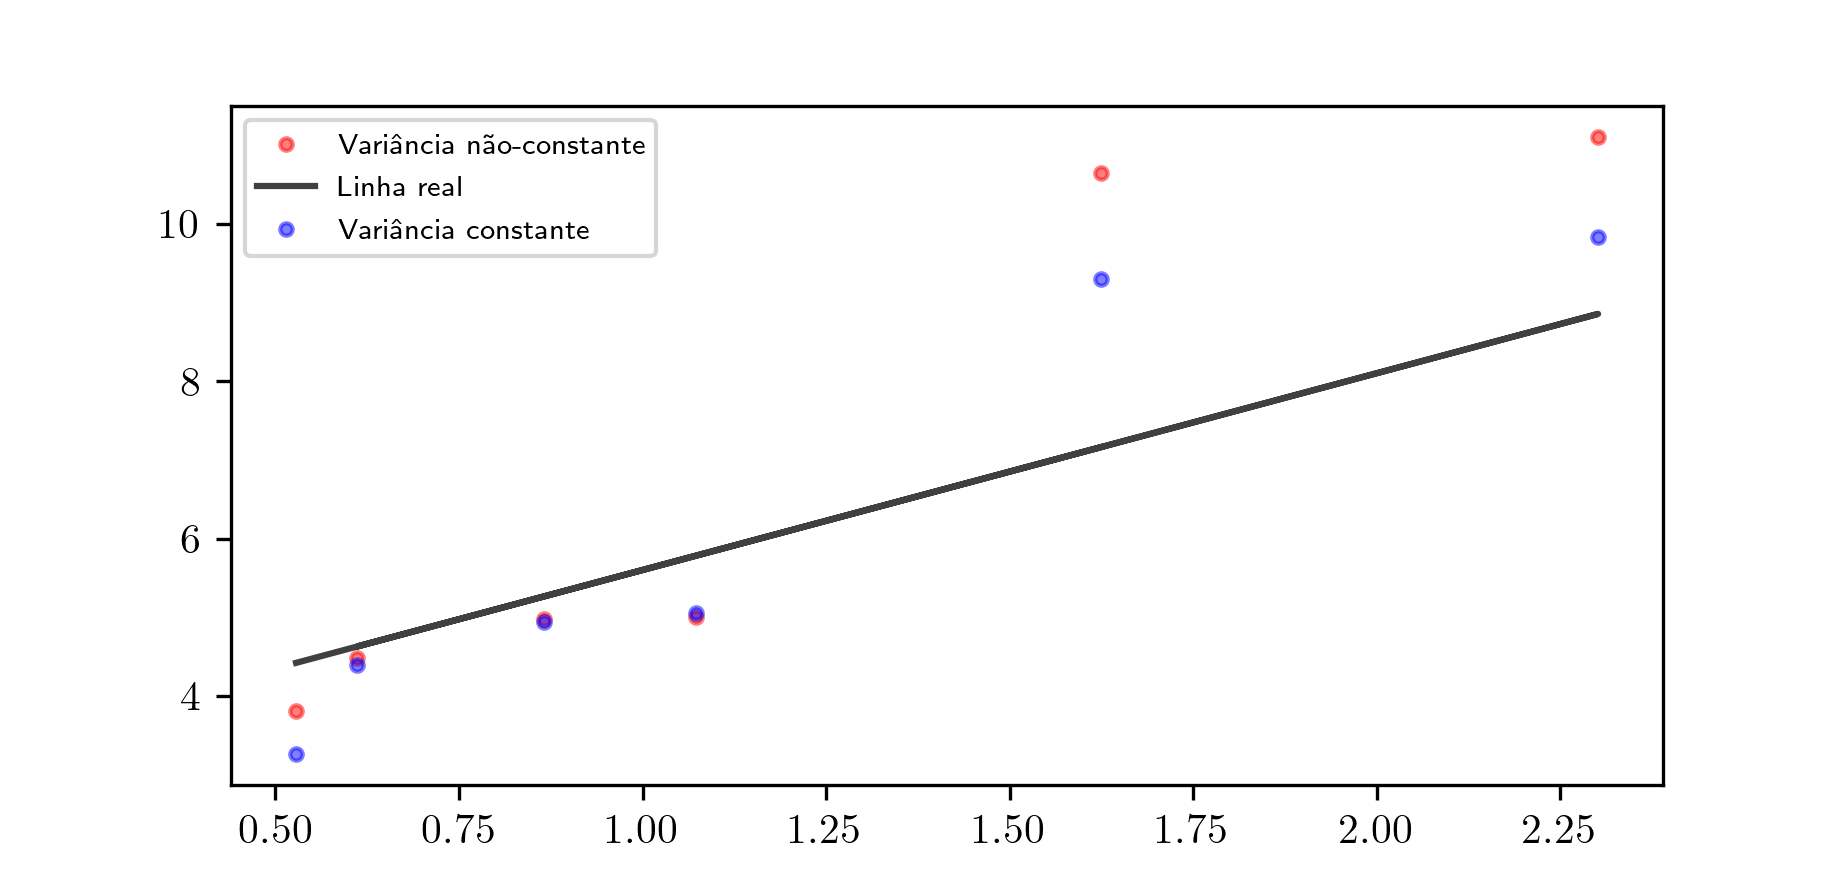
\includegraphics[width=12cm]{wls_var.png}
    \caption{Amostras com variância constante (azul) e amostras com variância não-constante (vermelho)}
    \label{fig:outlier}
\end{figure}

Em situações na qual essa premissa não é cumprida, é necessário adotar variâncias proporcionais:

\begin{equation}\label{eq:10}
Var(y_i|x_i) = \sigma^2 = \frac{1}{w_i}
\end{equation}

Onde $w_i$ são constantes de proporcionalidade, particulares a cada amostra.

De forma a utilizar deste recurso, é proposto o o método de linearização por mínimos quadrados ponderados  \cite{reg_analysis_weighted} \cite{weighted_taconeli}. Neste caso, a equação em estudo se apresenta de forma bastante semelhante ao método de mínimos quadrados ordinários, como pode ser observado na equação abaixo:

\begin{equation}\label{eq:11}
y_i = \alpha + x_i\beta +\epsilon_i^\ast
\end{equation}

Da mesma forma, $y_i$ representa o vetor de dados a serem estimados, $x_i$ representa o vetor de amostras, $\beta$ representa os coeficientes dependentes e $\alpha$ os independentes. A diferença está no $\epsilon^\ast$, que agora não mais representa erros com covariâncias constantes e sim, ao isolar $w_i$ na equação \ref{eq:10}, uma matriz de pesos denominada \textbf{W} da forma:

\begin{equation*}\textbf{W}=\left( \begin{array}{cccc} w_{1} & 0 & \ldots & 0 \\ 0& w_{2} & \ldots & 0 \\ \vdots & \vdots & \ddots & \vdots \\ 0& 0 & \ldots & w_{n} \\ \end{array} \right) \end{equation*}

Onde cada $w_i = \frac{1}{\sigma_i^2}$.

Assim, os valores de $\beta$ e $\alpha$ podem ser estimados à partir da soma dos quadrados dos erros $e_i^\ast$, da forma:

\begin{equation}\label{eq:12}
 \beta =\arg\min_{\beta}\sum_{i=1}^{n}\epsilon_{i}^{*2}\\ 
\end{equation}

Matricialmente, a equação \ref{eq:11} pode ser exposta como se segue:

\begin{equation}\label{eq:11matrix}
Y = \alpha + X\beta +\epsilon^\ast
\end{equation}

De forma um pouco mais detalhada, a equação \ref{eq:12} pode ser expandida da forma:

\begin{equation}\label{eq:13}
 S(\alpha,\beta) =\sum_{i=1}^{n} w_i(y_i - \alpha - \beta x_i)^2\\\ 
\end{equation}

Derivando como no método de mínimos quadrados ordinários, $\alpha$ e $\beta$ são equacionados:

\begin{equation}\label{eq:14}
 \alpha = \overline{y} - \beta \overline{x} 
\end{equation}

\begin{equation}\label{eq:15}
  \beta =\frac{\sum_{i=1}^{n}w_i(x_i - \overline{x})(y_i - \overline{y})}{\sum_{i=1}^{n} w_i(x_i - \overline{x})^2}\\\  
\end{equation}

Onde $\overline{x}$ e $\overline{y}$ são as médias ponderadas de \textit{x} e \textit{y}:

\begin{equation*}
  \overline{x} =\frac{\sum_{i=1}^{n}w_i x_i}{w_i}\\\  
\end{equation*}

\begin{equation*}
  \overline{y} =\frac{\sum_{i=1}^{n}w_i y_i}{w_i}\\\  
\end{equation*}

Matricialmente, representando $\textbf{X} = (x_i - \overline{x})$ e $\textbf{Y} = (y_i - \overline{y})$, a equação \ref{eq:15} é representada por:

\begin{align*} \beta =(\textbf{X}^{T}\textbf{W}\textbf{X})^{-1}\textbf{X}^{T}\textbf{W}\textbf{Y} \end{align*}

De forma gráfica, podemos comparar as duas formas de linearização por mínimos quadrados, para amostras com variância não-constante, através do exemplo exposto na figura \ref{fig:mqomqp}:

\begin{figure}[htp]
    \centering
    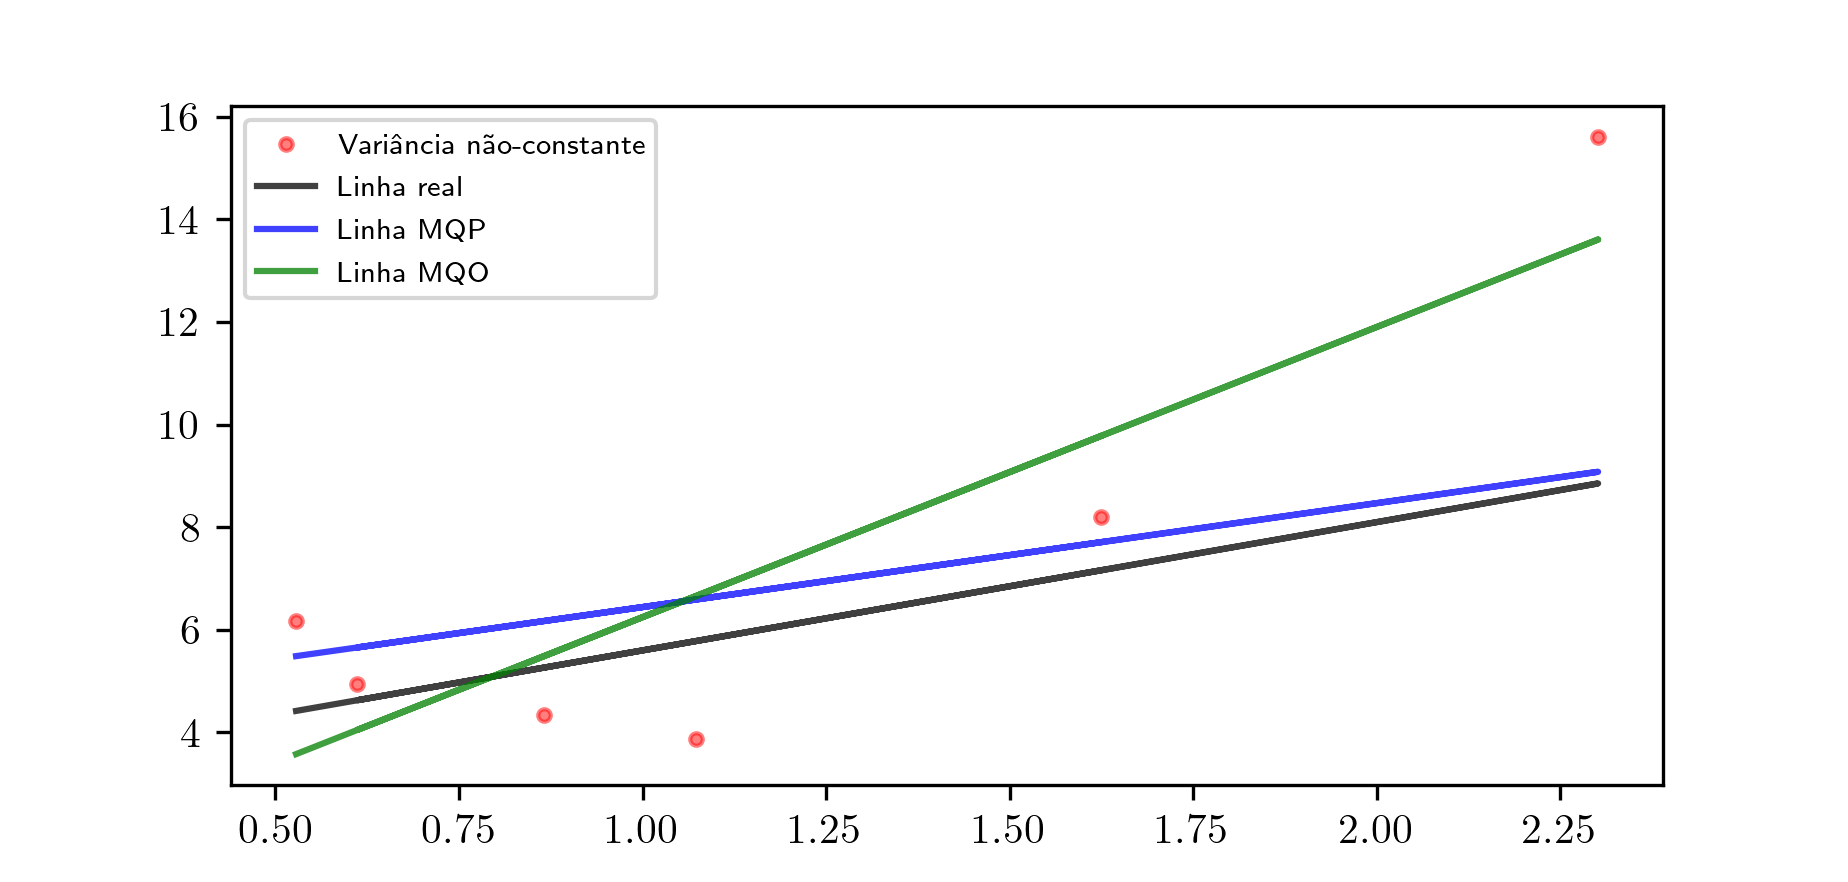
\includegraphics[width=12cm]{wls_fin.png}
    \caption{Linhas regressoras para o método dos Mínimos Quadrados Ordinários (MQO) e para o método dos Mínimos Quadrados Ponderados(MQP)}
    \label{fig:mqomqp}
\end{figure}

Como é facilmente perceptível, a linha regressora azul, referente ao resultado da linearização pelo método dos mínimos quadrados ponderados traz um erro associado significativamente menor que o observado na linha oriunda dos mínimos quadrados ordinários.

Uma das medidas de qualidade mais importantes para este tipo de regressão é o coeficiente de determinação $R^2$, que possui formulação bastante semelhante ao método de mínimos quadrados, segundo a análise de Willett e Singer \cite{r2_weighted}, diferindo apenas na soma total dos quadrados como equacionado abaixo:

\begin{equation}\label{eq:16}
R^2 = 1 - \frac{\sum_{i=1}^{n} y_i(\beta x_i + \alpha)^2}{\sum\limits_{i=1}^{n}{w_{i}y_{i}^{2}} - \frac{1}{\sum\limits_{k=1}^{n}w_{k}} \cdot \left(\sum\limits_{i=1}^{n}{w_{i}y_{i}} \right)^{2}.}
\end{equation}

Neste ponto, duas observações se fazem necessárias:

\begin{itemize}
  \item Uma vez que cada peso é inversamente proporcional à variância do erro, uma amostra com pequeno erro na variância terá um peso grande nas estimações;
  \item Os pesos deverão ser estimados (ou escolhidos arbitrariamente) considerando uma constante de proporcionalidade.
\end{itemize}

\section{Linearização por desvios mínimos absolutos - \textit{Least Absolute Deviations}}

Um dos principais pontos negativos de qualquer regressão linear por mínimos quadrados ocorre pois ao elevar ao quadrado o erro, é aumentada ao quadrado a importância das amostras com erro maior \cite{robust}. Isso pode ser particularmente prejudicial ao analisar \textit{outliers}, isto é, amostras discrepantes cujo erro pode não ter a mesma origem dos erros dos outros dados. Nestes casos, este método acabará priorizando estes valores discrepantes e isto aumentará o erro dos outros valores estimados.

Este fato é ilustrado na figura \ref{fig:infl_outlier}:

\begin{figure}[htp]
    \centering
    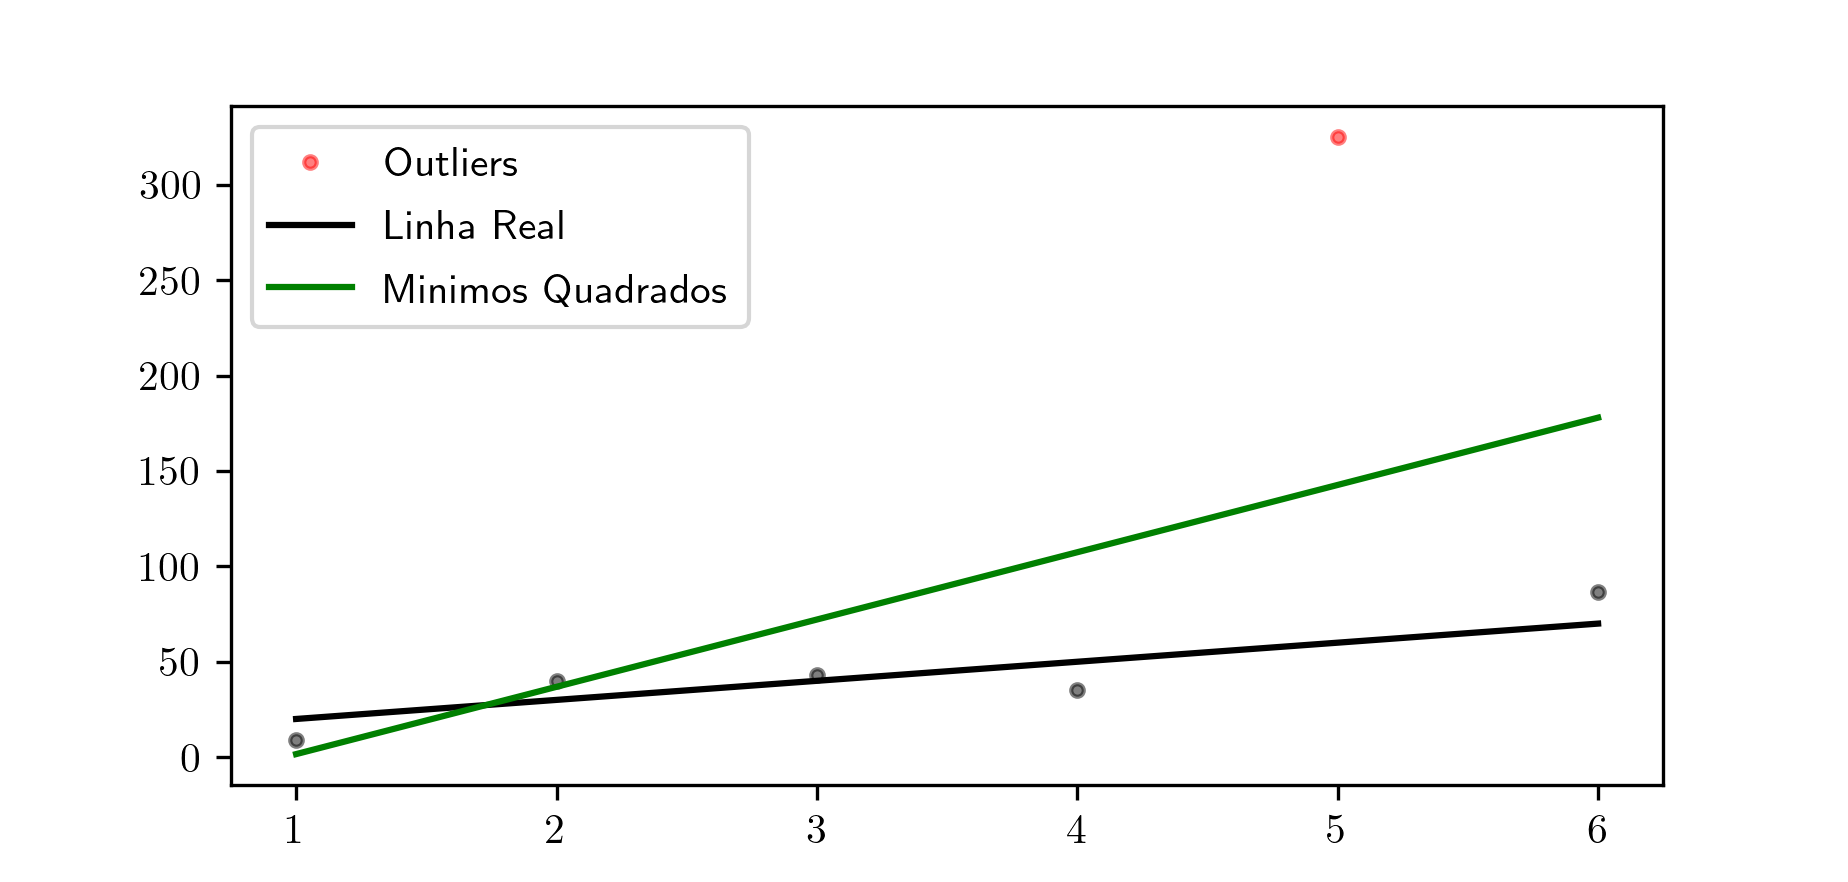
\includegraphics[width=12cm]{outlier_lsq.png}
    \caption{Influência de um \textit{outlier} na estimação dos valores de \textit{y} utilizando mínimos quadrados}
    \label{fig:infl_outlier}
\end{figure}

O \textit{outlier} (ponto em vermelho) faz com que o valor de $\beta$ aumente significativamente, inclinando a reta estimada por mínimos quadrados e aumentando o erro entre esta e os dados reais (pontos em cinza).

Visando reduzir este problema, a linearização por desvios mínimos absolutos é proposta pois a minimização neste caso é efetuada sobre o valor absoluto de $\epsilon$, em vez de $\epsilon^2$ \cite{lad}. Essa característica classifica este método de linearização como robusto\cite{robust}, isto é: mesmo que existam valores discrepantes entre as amostras, o método ainda será capaz de gerar uma solução com razoável eficiência.

Equacionando o $\beta$ para este método:

\begin{equation}\label{eq:17}
 \beta =\arg\min_{\beta}\sum_{i=1}^{n}|\epsilon_{i}|\\ 
\end{equation}

Substituindo $\epsilon$:

\begin{equation}\label{eq:18}
S(\alpha, \beta) = \sum_{i=1}^{n} |y_i - \alpha - \beta x_i|
\end{equation}

Para a implementação de um algoritmo que soluciona este método, é necessário ter em mente o fato de que a linha de regressão sempre cruza pelo menos dois pontos \cite{lad}. Tomando um primeiro ponto ($x_1$, $y_1$), deve-se buscar a melhor linha que passa através deste ponto. Esta linha deverá cruzar também outro ponto, ($x_2$, $y_2$). 

O próximo passo é procurar a melhor linha com respeito ao somatório de erros absolutos $\sum_{i=1}^{n}|\epsilon_{i}|$ que cruza ($x_2$, $y_2$). Essa linha cruzará, pelo menos, um outro ponto ($x_3$, $y_3$) e assim sucessivamente. Durante essa iterações, o valor de $\sum_{i=1}^{n}|\epsilon_{i}|$ diminui até que seja encontrada uma iteração com uma linha obtida idêntica a anterior, onde é possível concluir que esta é a melhor linha de regressão para os pontos fornecidos \cite{conciseenclyclopediaofstatistics}.

Para a construção da melhor linha cruzando ($x_1$, $y_1$), devemos encontrar o ponto ($x_k$, $y_k$) para qual a linha seja a melhor em termos de $\sum_{i=1}^{n}|\epsilon_{i}|$. Esta linha deverá ter a seguinte equação

\begin{equation}\label{eq:19}
y(x) = y_1 + \frac{y_k - y_1}{x_k - x_1} (x - x_1)
\end{equation}

Com a inclinação $\beta$:

\begin{equation}\label{eq:20}
\beta = \frac{y_k - y_1}{x_k - x_1}
\end{equation}

E com o deslocamento $\alpha$:

\begin{equation}\label{eq:21}
\alpha = y_1 - \beta x_1
\end{equation}

Para encontrar o ponto mais facilmente, são renomeados os (n - 1) pontos candidatos ${ \left(x_2,
	y_2\right), \ldots, \left(x_n,y_n\right) }$ de forma a obter:
	
\begin{equation*}
    \frac{y_2-y_1}{x_2-x_1} \leq \frac{y_3-y_1}{x_3-x_1}\leq \ldots \leq \frac{y_n-y_1}{x_n-x_1}\:
\end{equation*}

É definido também ${ T=\sum\limits_{i=1}^n \left|x_i-x_1\right| }$ para obter o ponto procurado em termos de \textit{k}, como se segue:

\begin{equation}\label{eq:22}
\begin{cases}
    \left|x_2-x_1\right| + \ldots + \left|x_{k-1}-x_1\right| & < \frac{T}{2} \\
    \begin{array}{l}\left|x_2-x_1\right| + \ldots \\+ \left|x_{k-1}-x_1\right| + \left|x_k-x_1\right|\end{array} & > \frac{T}{2}\:.
  \end{cases}
\end{equation}

Essa condição garante que $\beta$ minimize a equacão \ref{eq:23} de maneira análoga à $\sum_{i=1}^{n}|\epsilon_{i}|$ para as linhas de regressão passando por ($x_1$, $y_1$).

\begin{equation}\label{eq:23}
\sum_{i=1}^n\left| \left(y_i-y_1\right)-\beta\left(x_i-x_1\right)\right|
\end{equation}

É possível também verificar que a linha de regressão obtida passa pelo ponto ($x_k$,$y_k$), bastando apenas trocar o ponto ($x_k$,$y_k$) por ($x_2$,$y_2$) e recomeçar o algoritmo.


Utilizando os mesmos dados expostos na figura \ref{fig:infl_outlier}, a linearização por desvios mínimos absolutos traz o resultado exposto na figura \ref{fig:lad}:

\begin{figure}[H]
    \centering
    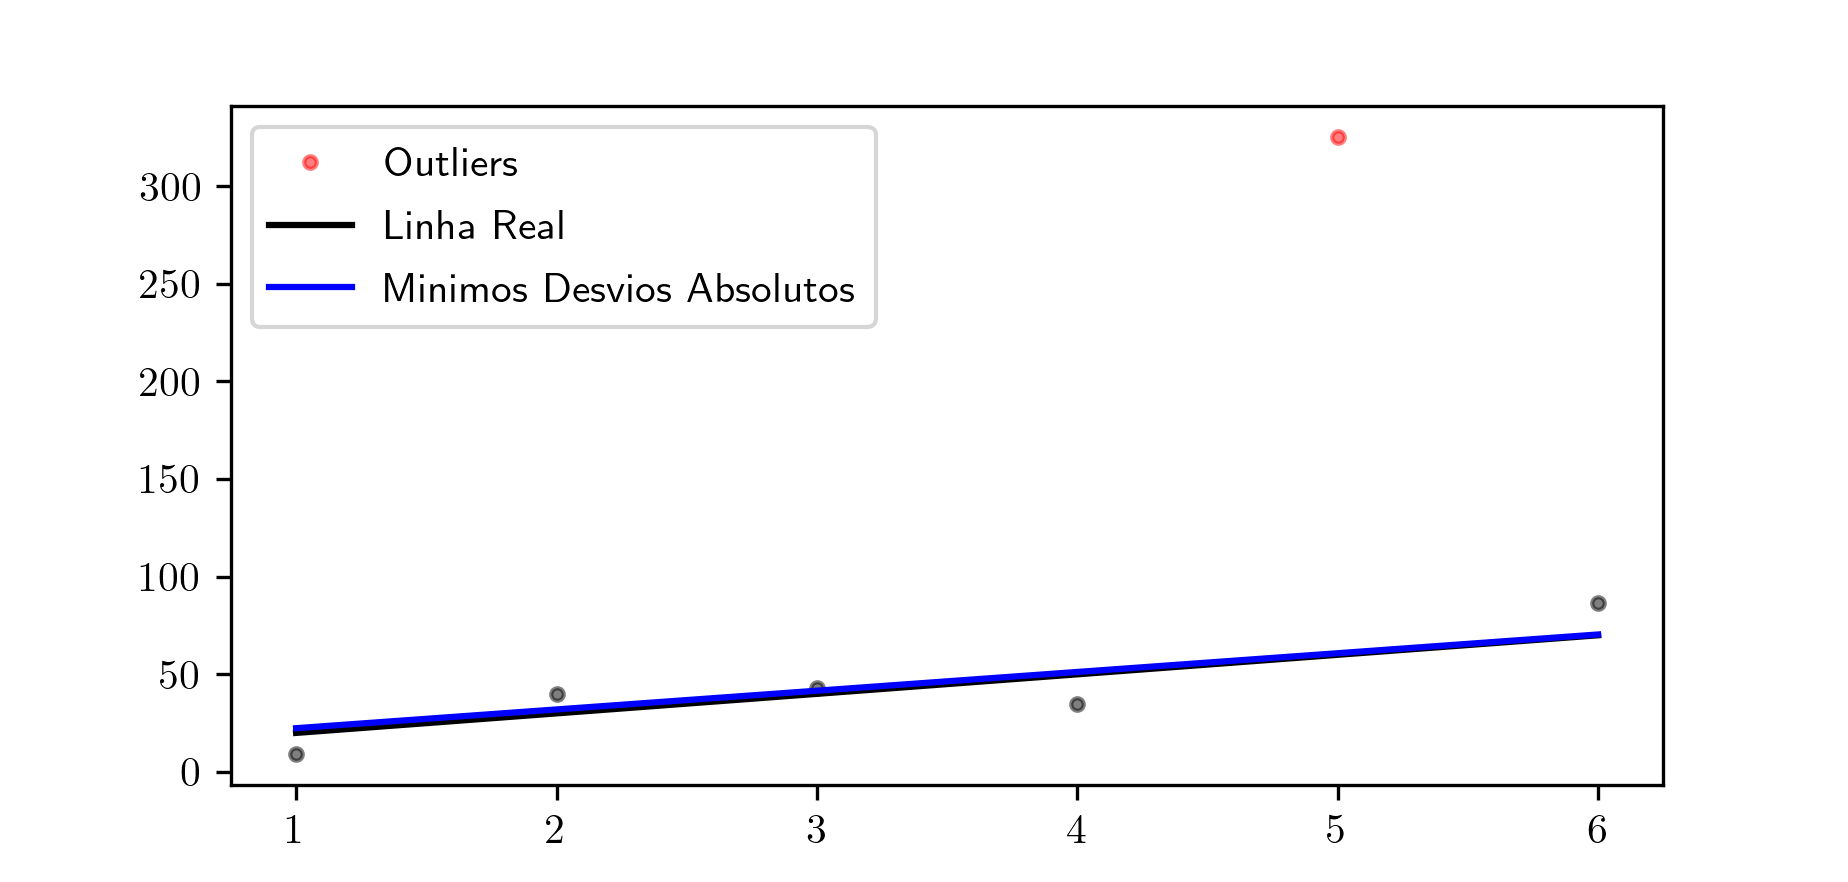
\includegraphics[width=12cm]{lad_ind.png}
    \caption{Linearização utilizando o método de desvios mínimos absolutos}
    \label{fig:lad}
\end{figure}

É facilmente observável o efeito dessa linearização: a linha de regressão estimada menospreza o \textit{outlier} em vermelho, mantendo os erros associados às outras amostras menores do que nos métodos de linearização anteriores.


Apesar destas grandes vantagens, este método possui algumas desvantagens consideráveis em relação aos anteriores, a saber:

\begin{itemize}
  \item Múltiplas soluções são possíveis;
  \item Uma ou mais soluções instáveis podem ser geradas pelo método. Isto é: a solução obtida poderá, para um pequeno ajuste no eixo \textit{y}, modificar a linha de regressão enormemente \cite{instabilitylad};
  \item Por ser um método essencialmente iterativo desde a estimação dos valores iniciais, uma maior quantidade de recursos computacionais se faz necessária.
\end{itemize}
